\section{Resultados}



\begin{frame}{Metodolog\'ia}
\begin{itemize}
    \item Par\'ametros principales de las configuraciones utilizadas:
        \begin{itemize}
            \item $\theta$
            \item $Max\_Axial\_Displacement$
            \item Uso de 1 o 3 pasos de la heur\'istica de asignaci\'on inicial
        \end{itemize}
    
    \item 12 Im\'agenes: 2 Sint\'eticas, 7 de Microt\'ubulos en {\it Arabidopsis Marchantia} y 3 de neuronas de rat\'on
    \begin{itemize}
        \item Caso evaluado por 2 expertos
    \end{itemize}
    
    %\item M\'etricas y Medidas:  VI, \'Indice Rand, \'Indice Jaccard
    \item Evaluaci\'on de:
        \begin{itemize}
            \item {\it Precision} y {\it Recall}
            \item N$\degree$ filamentos propuestos y correctos vs {\it ground truth}
        \end{itemize}
\end{itemize}
\end{frame}

\note[itemize]{
    \item Antes de discutir los resultados obtenidos, es necesario explicar los par\'ametros considerados. Dentro de los par\'ametros disponibles para personalizar el algoritmo propuesto, los principales par\'ametros utilizados en las pruebas fueron el umbral theta, el par\'ametro max axial displacement y el uso parcial o total de la heurística de asignaci\'on inicial debido a que estos par\'ametros fueron los que mostraron mayor impacto en los resultados
    \item Las pruebas considerar un total de 12 im\'agenes entre sint\'eticas y reales, con una imagen de microt\'ubulo de planta siendo evaluada por 2 expertos.
    \item La evaluaci\'on considera el n\'umero de filamentos propuestos as\'i como los filamentos correctos que indica el algoritmo propuesto, con respecto a lo indicado por un experto en cada caso. Esta informaci\'on se complementa con las medidas de precision y recall.
    
    %\item (SKIP) N$\degree$ Filamentos Propuestos y Correctos vs {\it Ground Truth}
    
    \item El resultado de la individualización de filamentos para cada imagen, consiste en el promedio de 10 iteraciones del algoritmo propuesto. Debido a que es un algoritmo que incluye c\'alculos de probabilidad, en cada iteraci\'on se cambia la semilla con la finalidad de explorar el espacio de b\'usqueda desde distintas partes.
}

% \begin{frame}{Im\'agenes Sint\'eticas}

%     \begin{figure*}[h]
%         \centering
%         \begin{subfigure}[t]{0.31\textwidth}
%             \centering
%             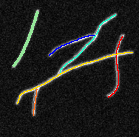
\includegraphics[height=1.3in]{Pictures/Synth-QuantitativeIFS-Fig7_groundTruth.png}
%         \end{subfigure}
%         ~ %\hspace{0.1cm}
%         \begin{subfigure}[t]{0.31\textwidth}
%             \centering
%             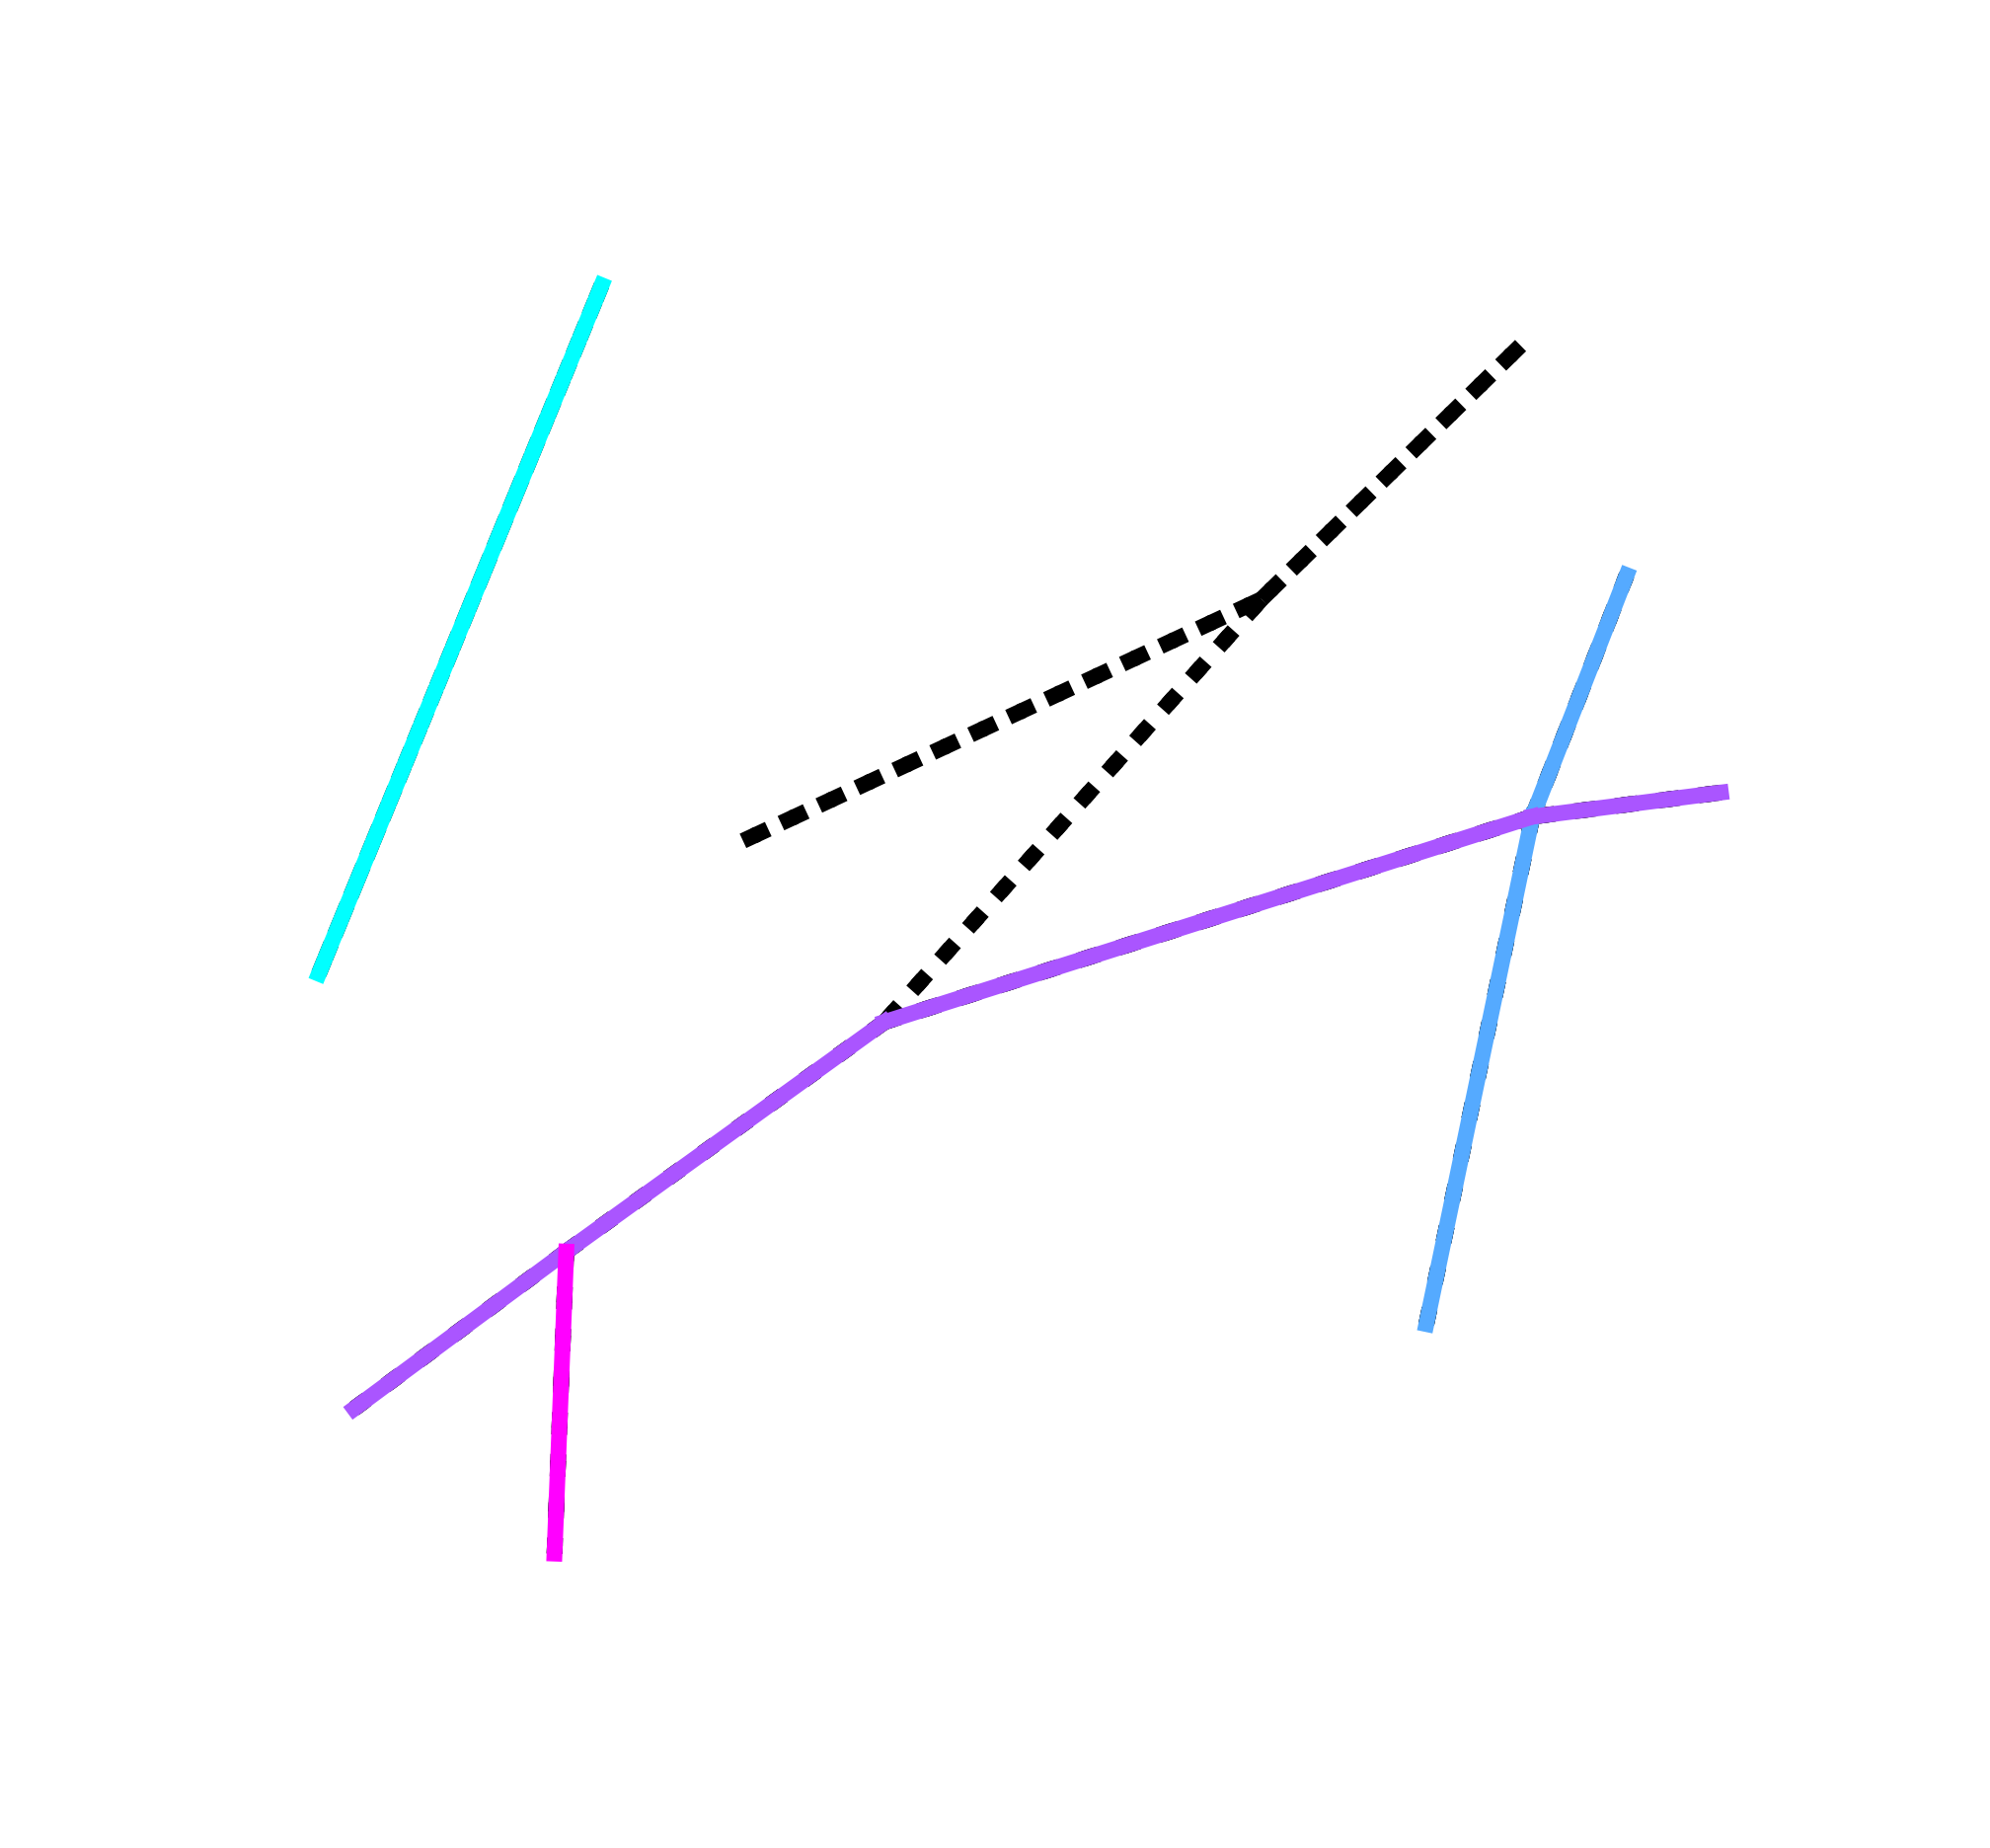
\includegraphics[height=1.3in]{Pictures/QFS7-DeFiNeExactMatch-30.png}
%         \end{subfigure}
%         ~
%         \begin{subfigure}[t]{0.31\textwidth}
%             \centering
%             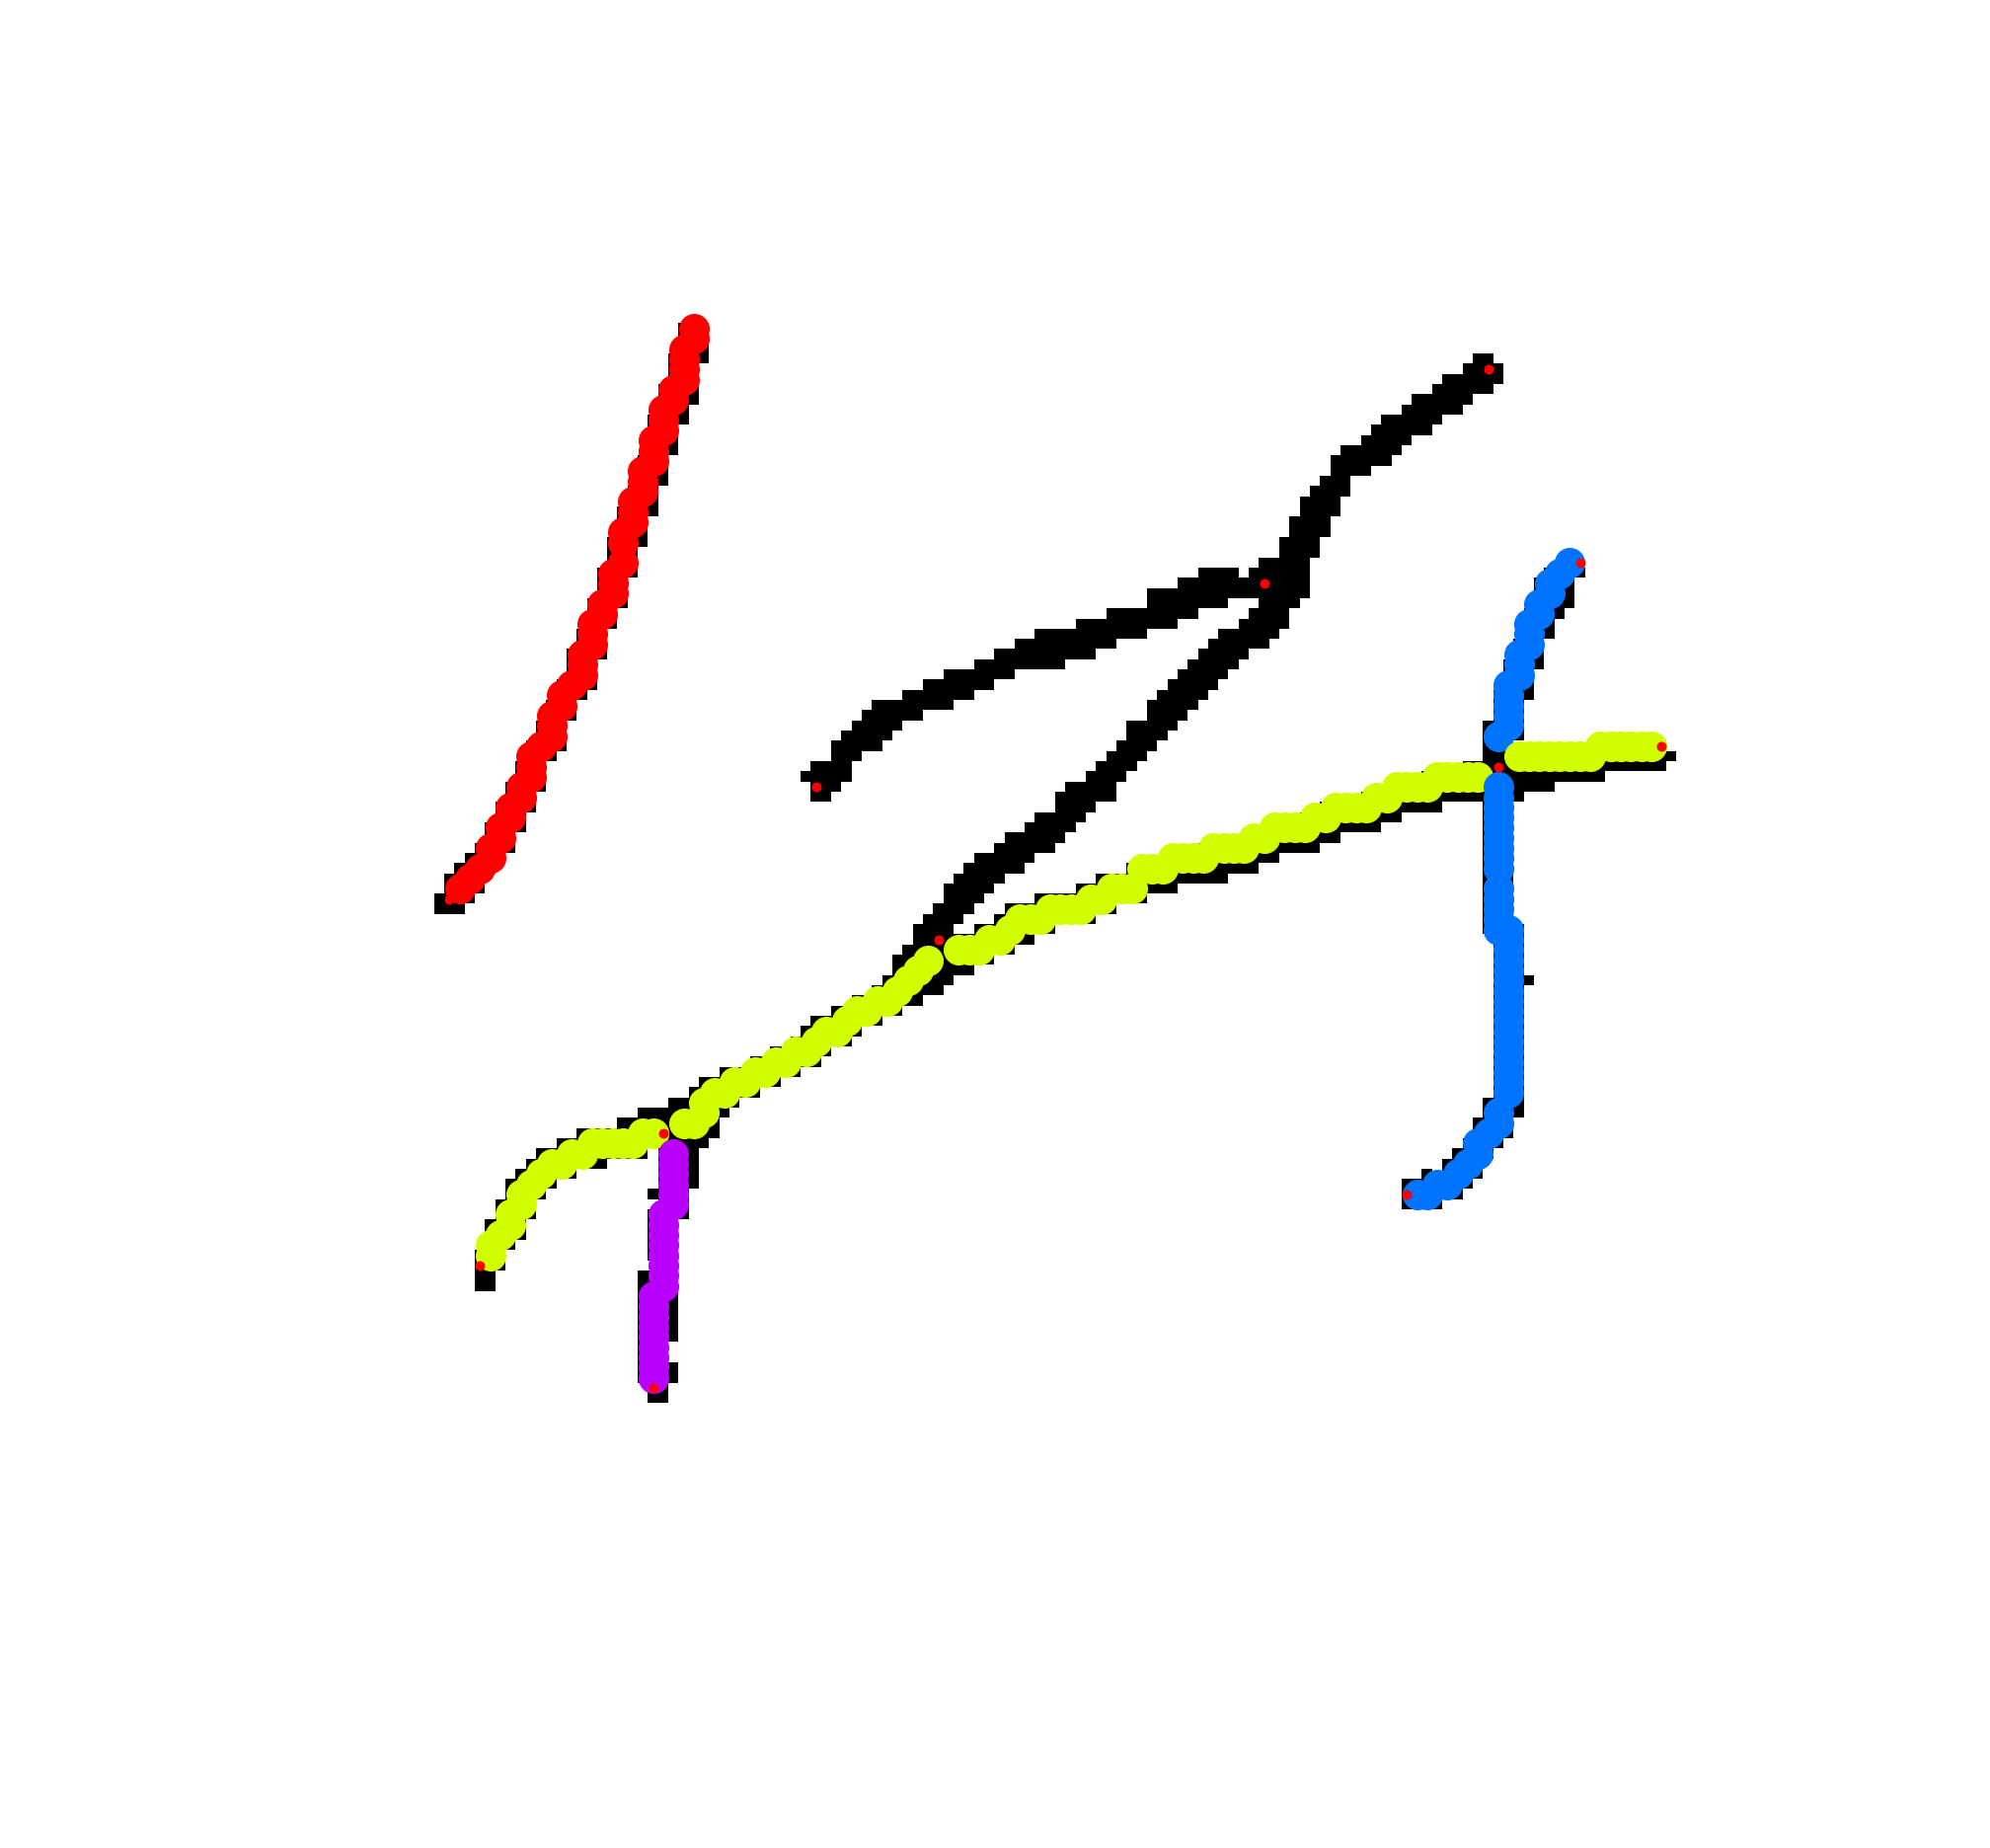
\includegraphics[height=1.3in]{Pictures/Synth-QuantitativeIFS-Fig7-phil-s1271-v056-exactMatch-antLabeled.png}
%         \end{subfigure}
%     \end{figure*}
    
% \resizebox{\textwidth}{!}{
%         %\footnotesize
%         \begin{tabular}{|c|c|c|c|c|c|c|c|c|c|c|c|c|}
%         \hline
%             Config & Iters & P & P* & R & R* & F1 & F1* & C/P & C/P* & C/GT & C/GT* & T[s]\\ \hline
%              DeFiNe 30\textdegree  & 1 & 0.72 & - & 0.47 & - & 0.57 & - & 4/6 & - & 4/6 & - & 2.3 \\
%              DeFiNe 60\textdegree & 1 &0.63 & - & 0.58 & - & 0.60 & - & 3/5 & - & 3/6 &- & 2.3\\
%             AP MT-P & 5 & 0.51 & 0.57 & 0.32 & 0.57 & 0.39 & 0.57 & 3/6.2 & 3/5 & 3/6 & 3/6 & 0.3\\
%             %Mejor Iteraci\'on P1 & 0.5714 & 0.5714 & 0.5714 & 3/5 &  & 0.3135 \\
%             AP S1 & 5 & 0.68 & 0.87 &0.57 & 1 & 0.62 & 0.93 & 4/5.8 & 4/5 & 4/6 & 4/6 & 0.2\\
%             % {\bf Mejor Iteraci\'on P2} & 0.875 & 1 & 0.9333 & 4/5 & 4/6 & 0.3073\\
%              \hline
%         \end{tabular}
%     }
% \end{frame}

\begin{frame}{Im\'agenes Sint\'eticas (OE 4)}
    \vspace{-0.6cm}
    \begin{columns}
        \begin{column}{0.31\textwidth}
        
            \begin{figure}
                \centering
                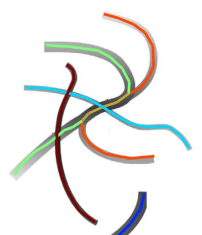
\includegraphics[height=1.3in]{Pictures/define-weighted-4-groundTruth.png}
                \caption{Ground Truth}
            \end{figure}
        \end{column}
        \begin{column}{0.31\textwidth}
        %\vspace{-1cm}
            \begin{figure}
                \centering
                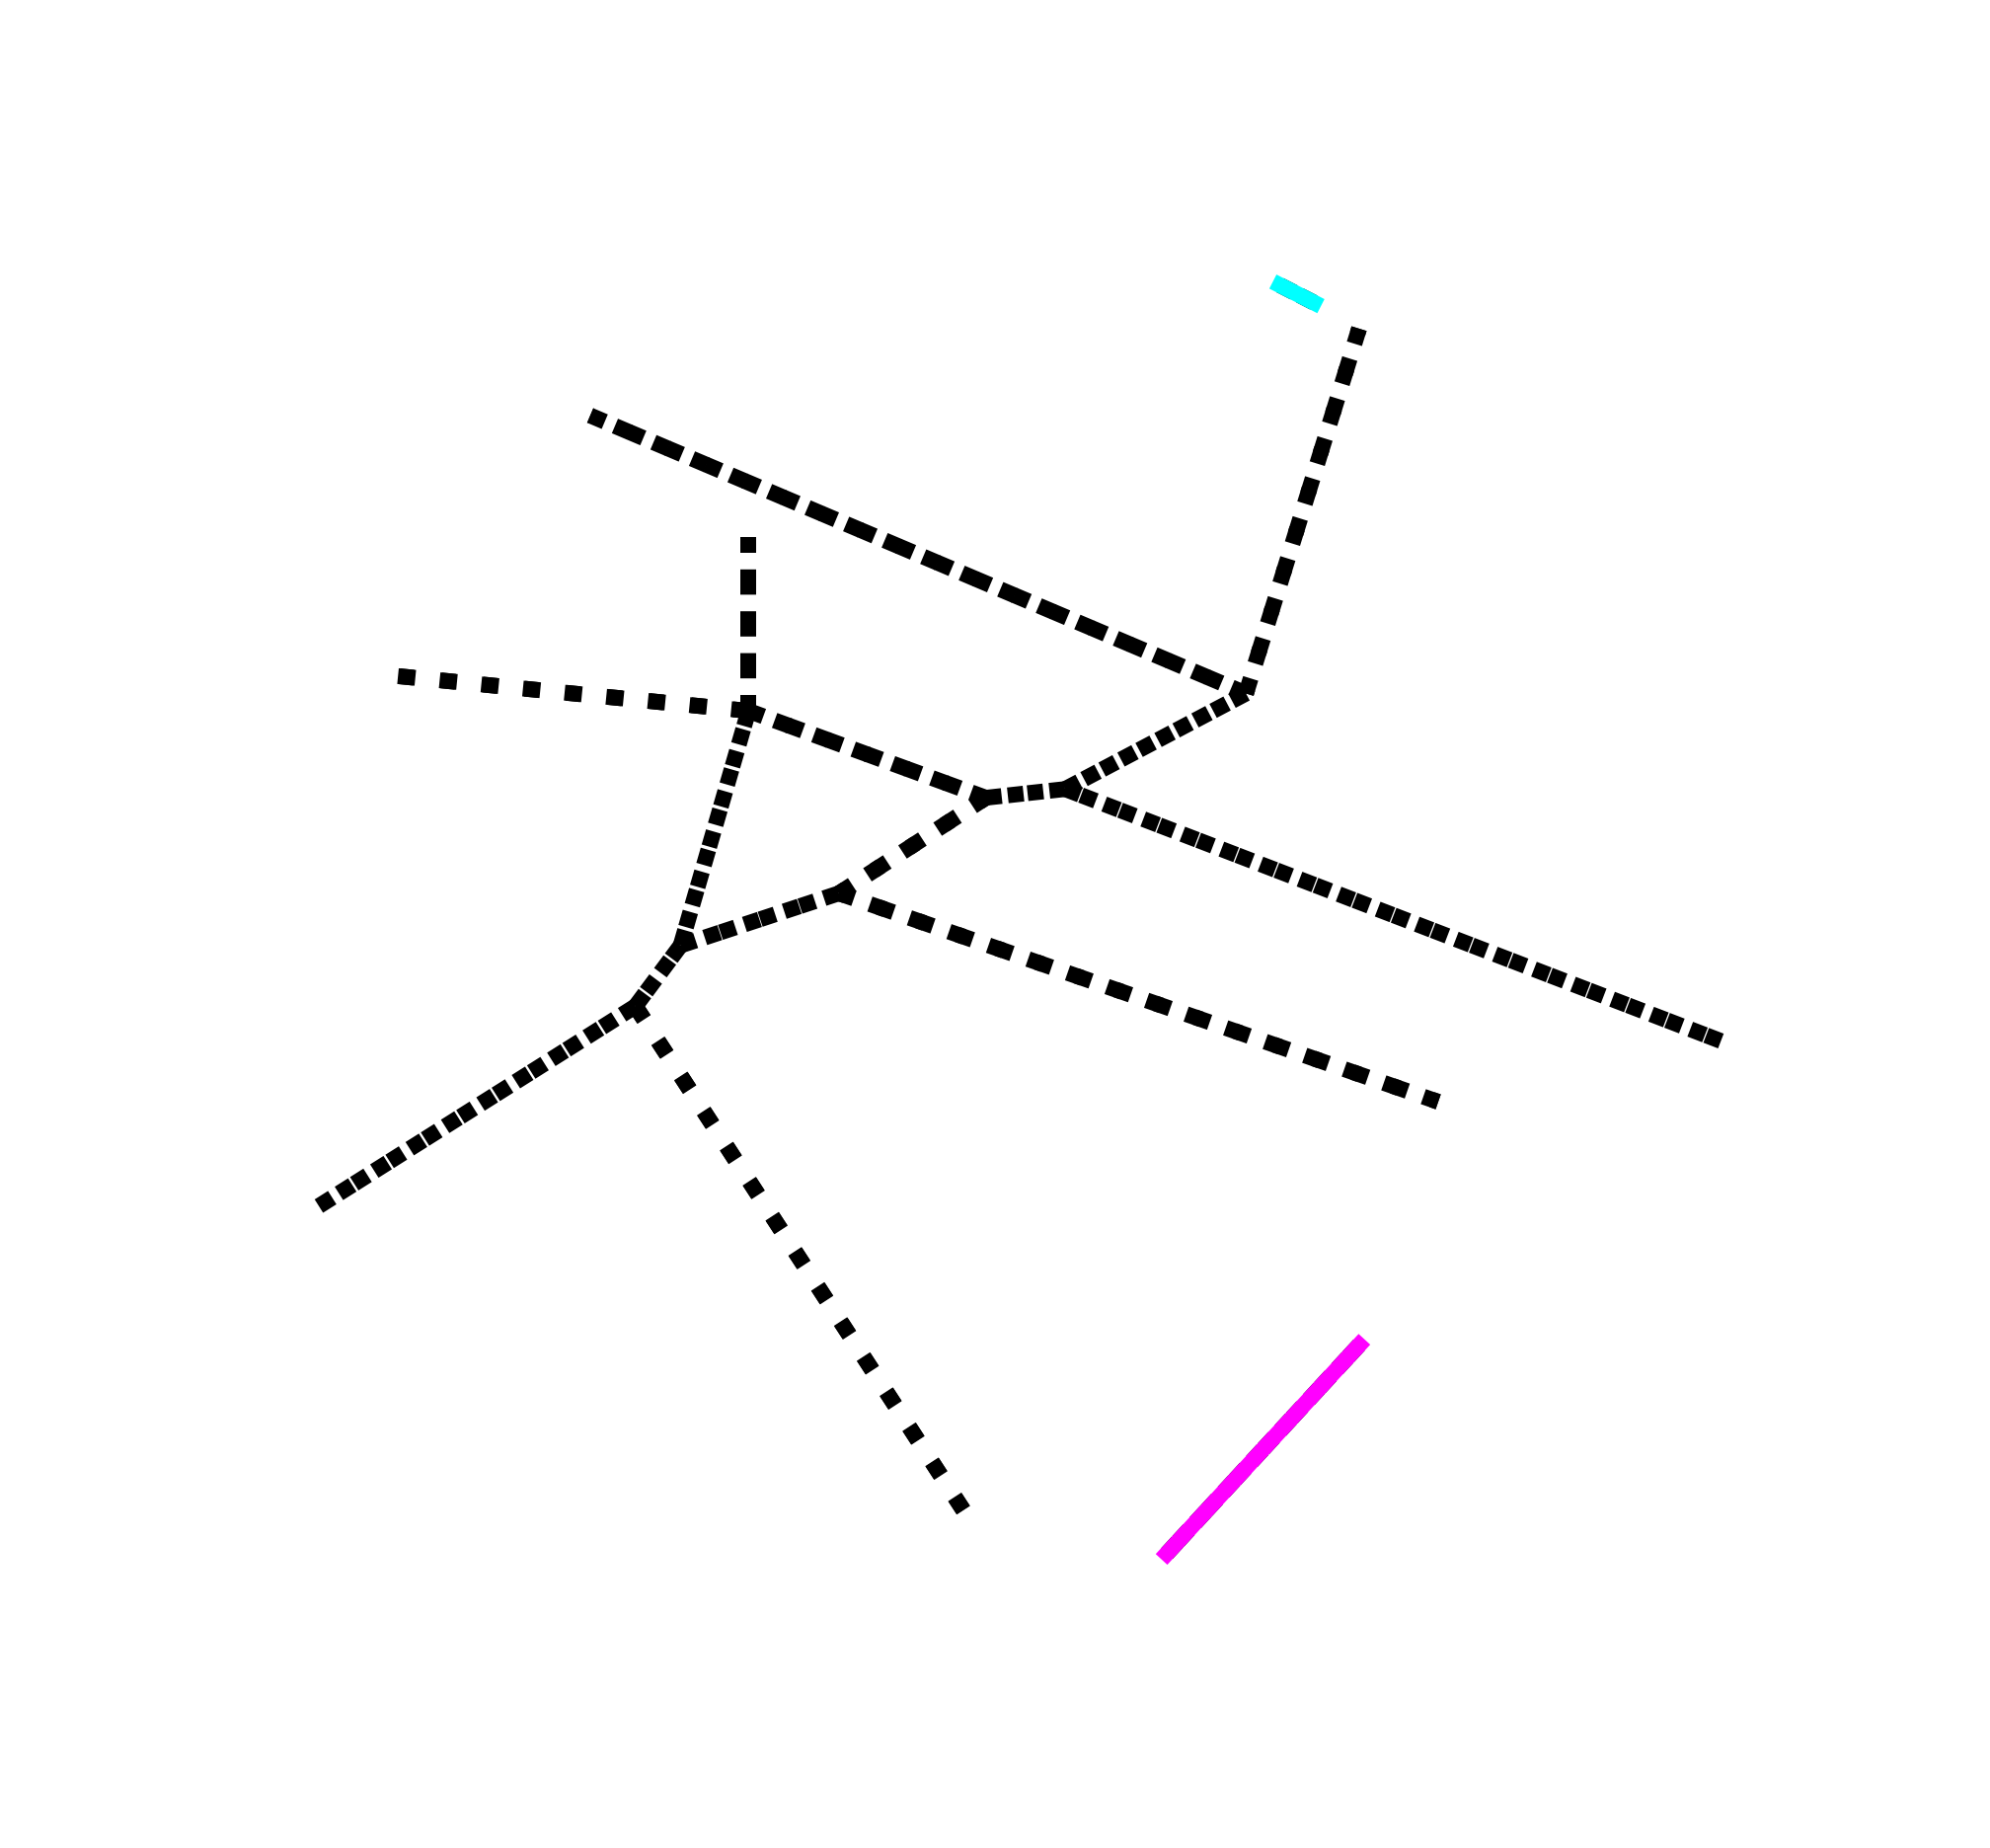
\includegraphics[height=1.3in]{Pictures/defineFig1b-DeFiNeExactMatch-30.png}
                \caption{DeFiNe 30\textdegree}
            \end{figure}
        \end{column}
        \begin{column}{0.31\textwidth}
        %\vspace{-1cm}
            \begin{figure}
                \centering
                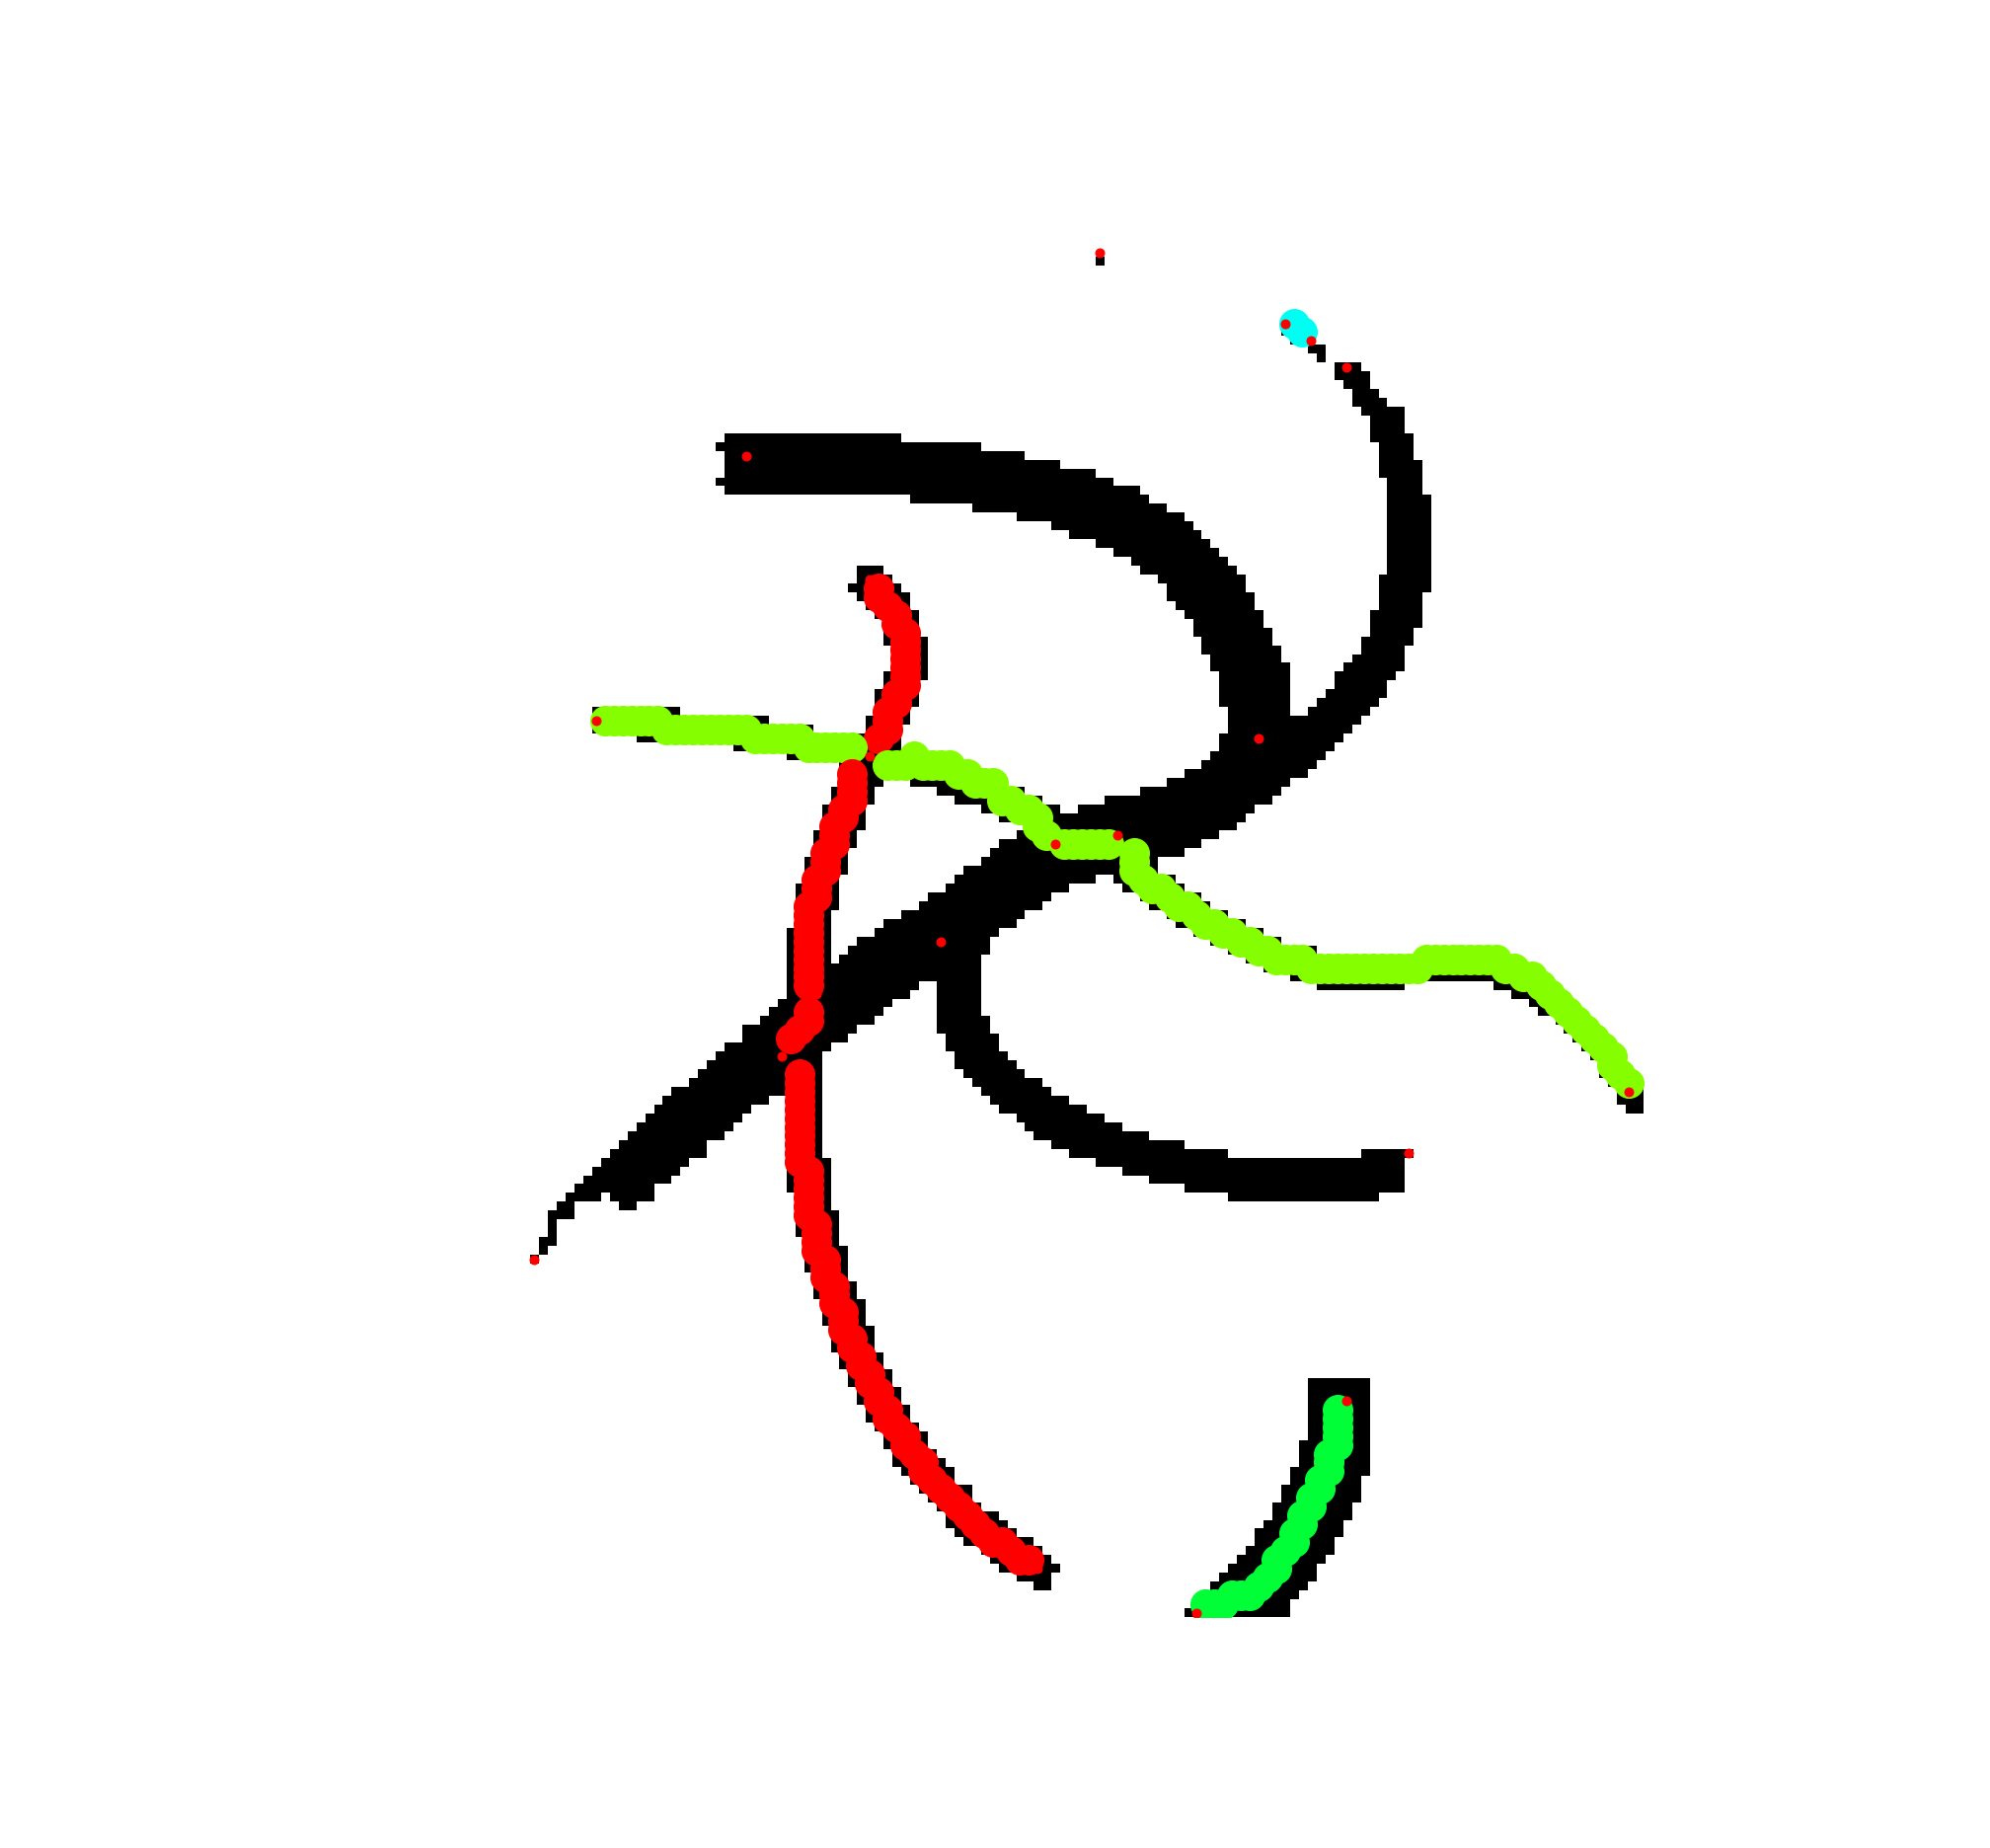
\includegraphics[height=1.3in]{Pictures/define-weighted-4-phil-s3389-v056-exactMatch-antLabeled.png}
                \caption{AP S2}
            \end{figure}
        \end{column}
    \end{columns}

    \vspace{-0.3cm}
    \begin{table}[h]
    \resizebox{0.85\textwidth}{!}{
        \begin{tabular}{|c|c|c|c|c|c|c|c|c|}
        \hline
        Config & Iters & P & R & C/P & C/P* & C/GT & C/GT* & T[s] \\ \hline
        DeFiNe 30\textdegree & 1 & 0.33 & 0.18 & 2/11 & - & {\bf 2/5} & - & 2.8 \\
        DeFiNe 60\textdegree & 1& 0.23 & 0.25 & 2/7 & - & 2/5 & - & 3.6\\
        AP MtP & 10 & 0.34 & 0.27 & 3/9.2 & 3/9 & 3/6 & 3/6 & 0.3\\
        AP S2 & 10 & 0.32 & 0.25 & 4/8.6 & 4/9 & {\bf 4/6} & 4/6 & 0.3\\
            \hline
        \end{tabular}
    }
    \caption{(*) indica el mejor resultado de las 10 iteraciones.}
    \end{table}
\end{frame}

\note[itemize]{
\scriptsize
  \item A modo de ejemplo para las imagenes sint\'eticas evaluadas, se presenta una imagen sint\'etica que contiene 5 filamentos. El grafo que representa estos 5 filamentos esta compuesto por 17 aristas.
  
  %\item esta imagen sintetica se obtiene del paper de Define

 \item Para DeFiNe, se consideran 2 configuraciones id\'enticas basadas en los mejores resultados obtenidos por esa herramienta de acuerdo a sus autores, y s\'olo se varia el \'angulo de umbral de BFS, mientras que con el algoritmo propuesto se utilizaron 2 configuraciones, una predeterminada para microt\'ubulos de planta, definida como MtP y otra personalizada definida como S2
 
 \item Tanto para DeFiNe como para el algoritmo propuesto, los resultados de precision y recall no son muy elevados. Sin embargo se observa que ambas configuraciones del algoritmo propuesto tienen un comportamiento similar.
 
 \item En particular, en la 5ta columna, C vs P, que representa los filamentos correctamente identificados versus el n\'umero de filamentos propuestos, la configurac\'on predeterminada para microt\'ubulo de planta logra identificar correctametne 3 filamentos de los 9 que propone, mientras que la configuraci\'on S2, que tiene ajustes particulares para esta imagen, obtiene una identificaci\'on correcta adicional, y a la vez reduce el promedio de filamentos propuestos.
 
 \item Una de las modificaciones de la configuraci\'on S2 con respecto a la de microt\'ubulos es que S2 solo utiliza el primer criterio en la heur\'istica de asignaci\'on inicial de aristas, ya que este caso sint\'etico no contiene filamentos que nacen a partir de otros.
 %\item La idea principal es que el n\'umero de filamentos correctamente identificados sea sino identico, lo m\'as cercano al n\'umero de filamentos propuestos, ya que 
 
 
 \item Es necesario mencionar que en las columnas C vs GT, que representan los filamentos identificados correctamente con respecto a lo definido por un experto, se consideran 6 filamentos como ground truth para el algoritmo propuesto  debido a que la herramienta que genera el grafo para el algoritmo propuesto gener\'o una arista aislada en la parte superior, que realmente corresponde a la continuaci\'on de una arista y no a otra por si sola. 
 
 \item En la visualizaci\'on de los filamentos identificados por el algoritmo propuesto, a la derecha de la presentaci\'on, se observa que los filamentos no identificados corresponden a los que presentan una mayor curvatura.
 Es probable que con una configuraci\'on m\'as afinada, el algoritmo propuesto pueda encontrar los 2 filamentos faltantes, ya que ese comportamiento se aleja un poco de lo observado en los filamentos incluidos en este trabajo.
}

\begin{frame}{Muestra MT-A Microt\'ubulo (OE 4)}
\vspace{-1cm}
    \begin{columns}
        \begin{column}{0.22\textwidth}
            \begin{figure}
                \centering
                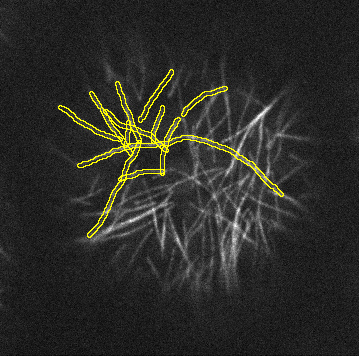
\includegraphics[height=1.3in]{Pictures/SPINNING-DISK-MARCHANTIA-rois-unlabeled.png}
                \caption{Imagen Original}
            \end{figure}
        \end{column}
        \begin{column}{0.22\textwidth}
            \begin{figure}
                \centering
                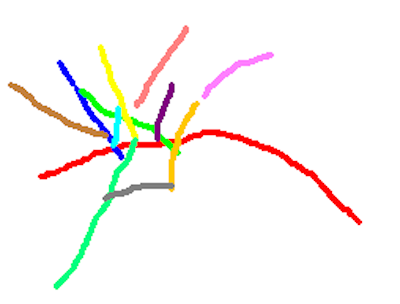
\includegraphics[height=1.3in]{Pictures/50-ROIs-Spinning-Marchantia-solved-rot-unlabeled.png}
                \caption{Ground Truth}
            \end{figure}
        \end{column}
        \begin{column}{0.22\textwidth}
            \begin{figure}
                \centering
                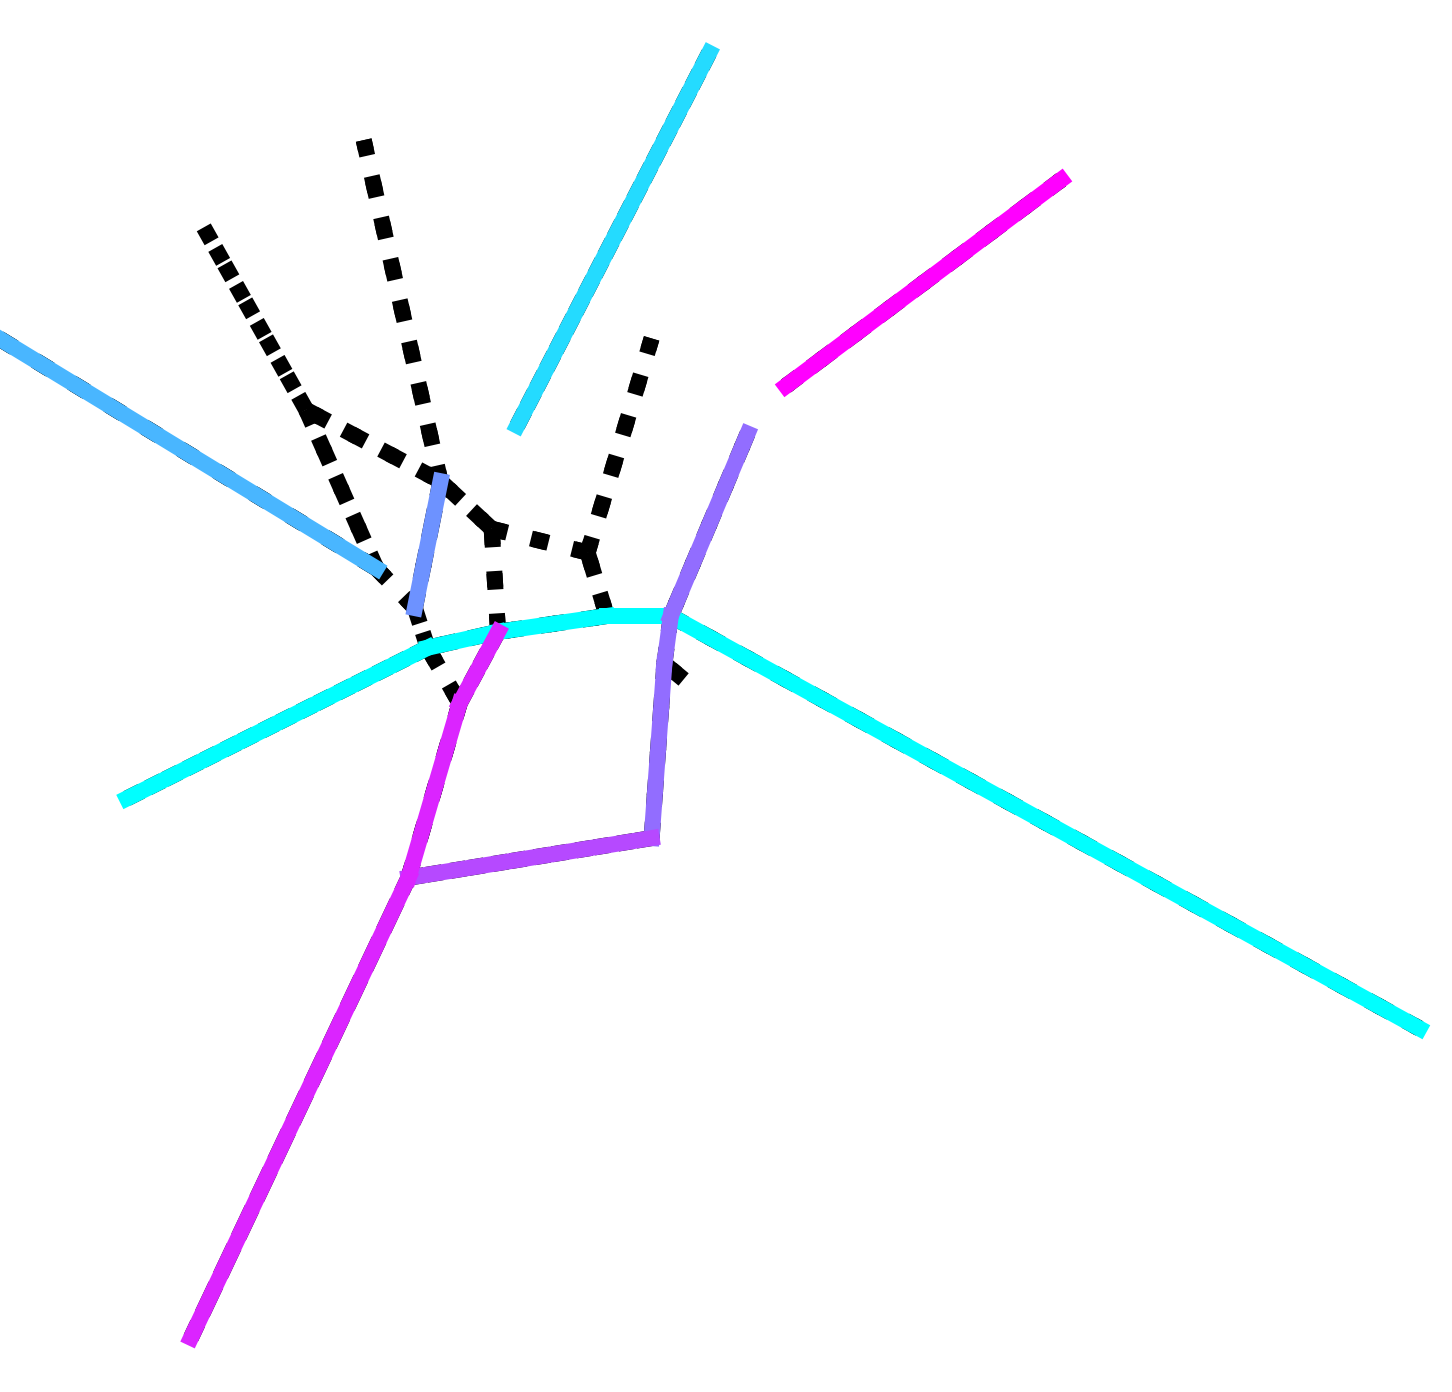
\includegraphics[height=1.3in]{Pictures/50-ROIs-Spinning-Marchantia-DeFiNeExactMatch-30.png}
                \caption{DeFiNe 30\textdegree}
            \end{figure}
        \end{column}
        \begin{column}{0.22\textwidth}
            \begin{figure}
                \centering
                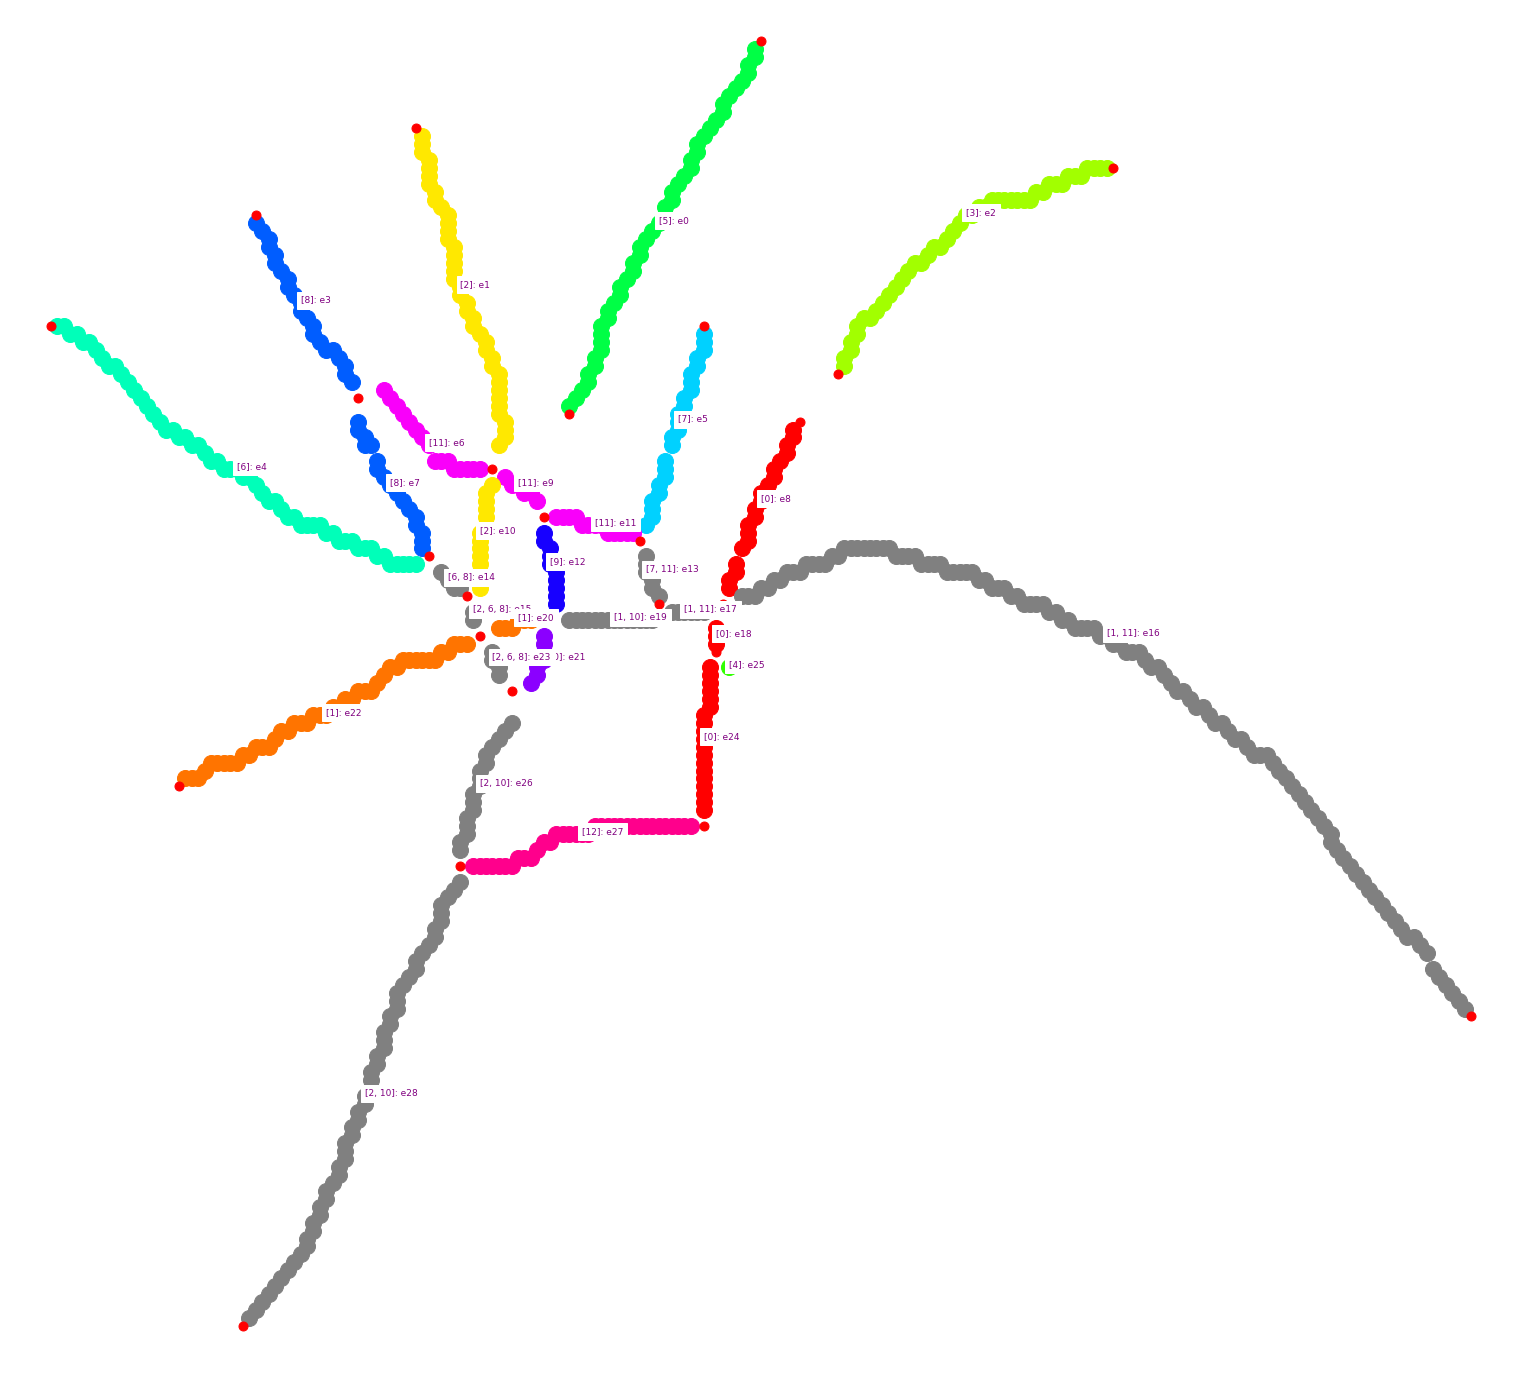
\includegraphics[height=1.3in]{Pictures/50-ROIs-Spinning-Marchantia-phil-s10-v05-nobg-antLabeled.png}
                \caption{AP S2}
            \end{figure}
        \end{column}
    \end{columns}

    \begin{table}[h]
    \resizebox{0.85\textwidth}{!}{
        \begin{tabular}{|c|c|c|c|c|c|c|c|c|c|c|}
        \hline
              Config & Iters & P & R & C/P & C/P* & C/GT & C/GT* & T[s] \\ \hline
             DeFiNe 30\textdegree & 1 & 0.65 & 0.45 & 8/16 & - & {\bf 8/12} & - & 4.1 \\
             DeFiNe 60\textdegree & 1& 0.28 & 0.21 & 3/12 &- & 3/12 & - & 3.6\\
            AP MT-P & 10 & 0.44 & 0.34 & 7.2/12.4 & 8/13 & 7.2/12 & {\bf 8/12} & 0.3\\
             \hline
        \end{tabular}
        }
    \caption{Grafo de 29 aristas}
    \end{table}
\end{frame}

\note[itemize]{
  \item grafo de 29 aristas
}

\begin{frame}{Neuronas de rat\'on (OE 4)}
%\vspace{-1cm}
    \resizebox{\textwidth}{!}{
        \begin{tabular}{|c|c|c|c|c|r|c|}
        \hline
             Muestra & Algoritmo & Fil. Propuestos & {\it GT} &\% Asignaci\'on & Tiempo[s] & N\textdegree~ Aristas\\
             \hline
             \multirow{3}{*}{N1}& DeFiNe 30\textdegree & 246 & \multirow{3}{*}{24} &100 & 1514.6 & \multirow{3}{*}{414} \\
                    & DeFiNe 60\textdegree & 192 && 100 & 15573.7 &\\
                    & AP N Promedio & 59 && 53.7 & 32.5 &\\ \hline
            \multirow{3}{*}{N2}& DeFiNe 30\textdegree & 113 & \multirow{3}{*}{29} & 100 & 82.2 & \multirow{3}{*}{161}\\
                    & DeFiNe 60\textdegree & 85 && 100 & 456.4 &\\
                    & AP N Promedio & 34.8 && 59.3 & 4.9 &\\ \hline
            N3 & AP N Promedio & 17.4 & 14 & 57.8 & 4.2 & 67\\ \hline
        \end{tabular}
    }
    \vspace{0.5cm}
    \begin{itemize}
        \item \% Asignaci\'on debe estar relacionado a la calidad de la informaci\'on, evitando asignar s\'olo por cumplir con el modelo
        \item N\textdegree~ Fil. Prop. refleja acotamiento del espacio de b\'usqueda
    \end{itemize}
\end{frame}

\note[itemize]{
\small
  \item En las neuronas de raton, las pruebas ejecutadas con DeFiNe presentan cantidades de filamentos propuestos 2 a 6 veces mayores que el n\'umero de filamentos individualizados por un experto. Este comportamiento puede atribuirse a la obligaci\'on que DeFiNe tiene de asignar todas las aristas al menos a un filamento. En comparaci\'on, el algoritmo propuesto al tener mayor flexibilidad, asigna en promedio un 57\% de las aristas a filamentos.
  
  \item Adicionalmente, los tiempos de ejecuci\'on de las pruebas con DeFiNe son sustancialmente mayores, encontr\'andose en el rango de los minutos a las 4 horas, dependiendo de los par\'ametros utilizados. Lo anterior puede asociarse al n\'umero de aristas que las muestras de neurona tienen en su respectivo grafo
  
  \item En cuanto al algoritmo propuesto, a pesar de ejecutar todas las evaluaciones en tiempos menores a 40 segundos, las individualizaciones correctas son bajas, mientras que el n\'umero de filamentos propuestos se acerca a la cantidad de filamentos individualizados manualmente por un experto, exceptuando el caso de la Muestra N1.
  
  \item  Es posible asociar un comportamiento razonable del n\'umero de filamentos propuestos con la restricci\'on especial para neuronas considerada dentro de las penalizaci\'on de anti-feromonas, lo que permite mantener acotado el n\'umero de filamentos propuestos mediante el descarte de soluciones infactibles.
}

\begin{frame}{Muestra N3 de neurona de rat\'on (OE 4)}
    \vspace{-0.2cm}
        \begin{columns}
        \begin{column}{0.45\textwidth}
            \begin{figure}
                \centering
                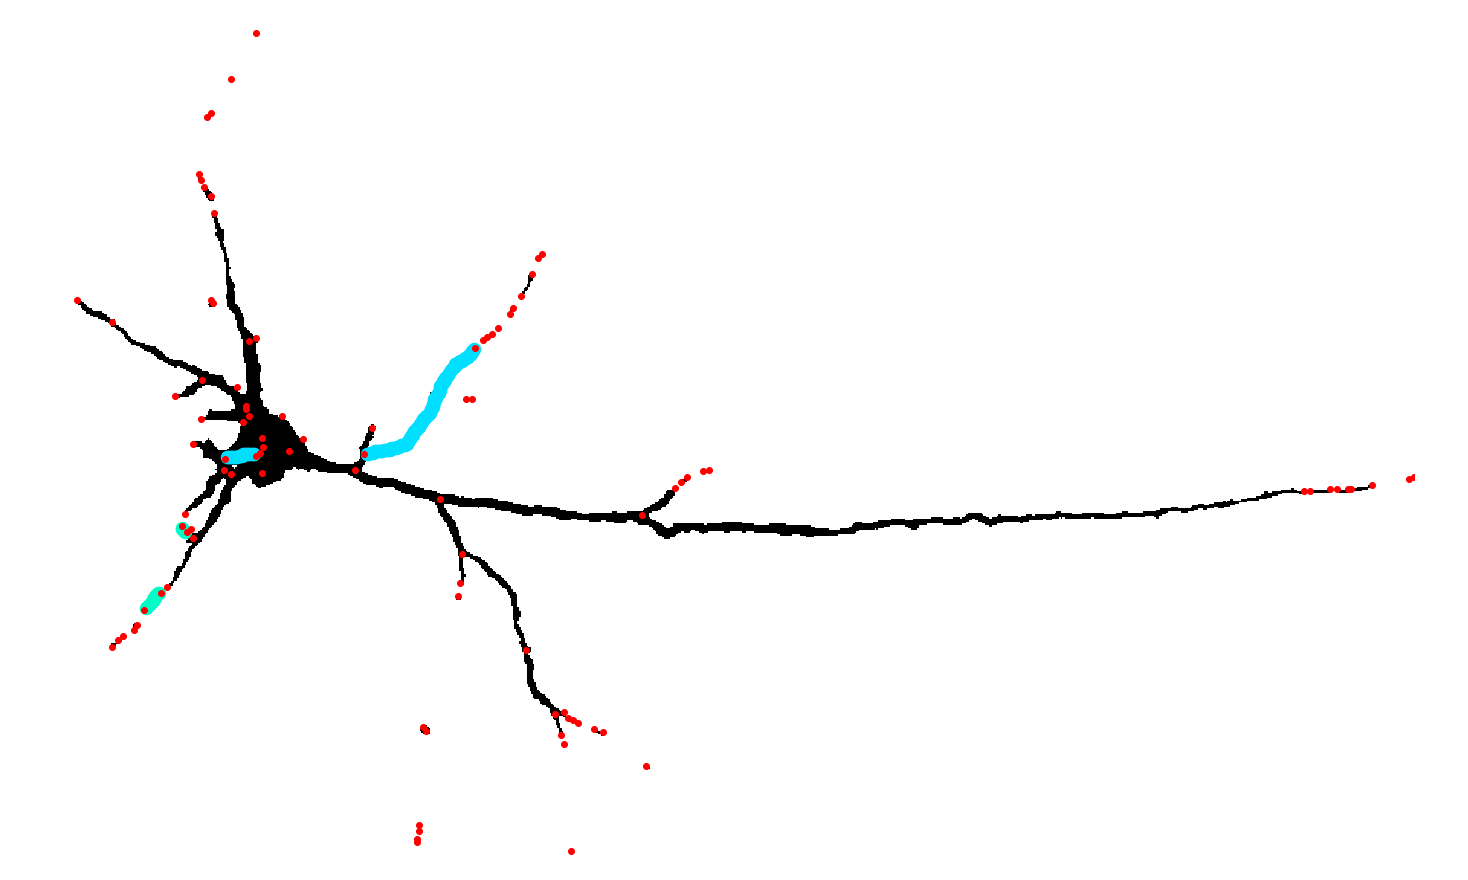
\includegraphics[height=1.35in]{Pictures/Porta18-3a1-phil-s10-v056-exactMatch-antLabeled.png}
                \caption{Muestra N3 Calce Exacto}
            \end{figure}
        \end{column}
        \begin{column}{0.45\textwidth}
            \begin{figure}
                \centering
                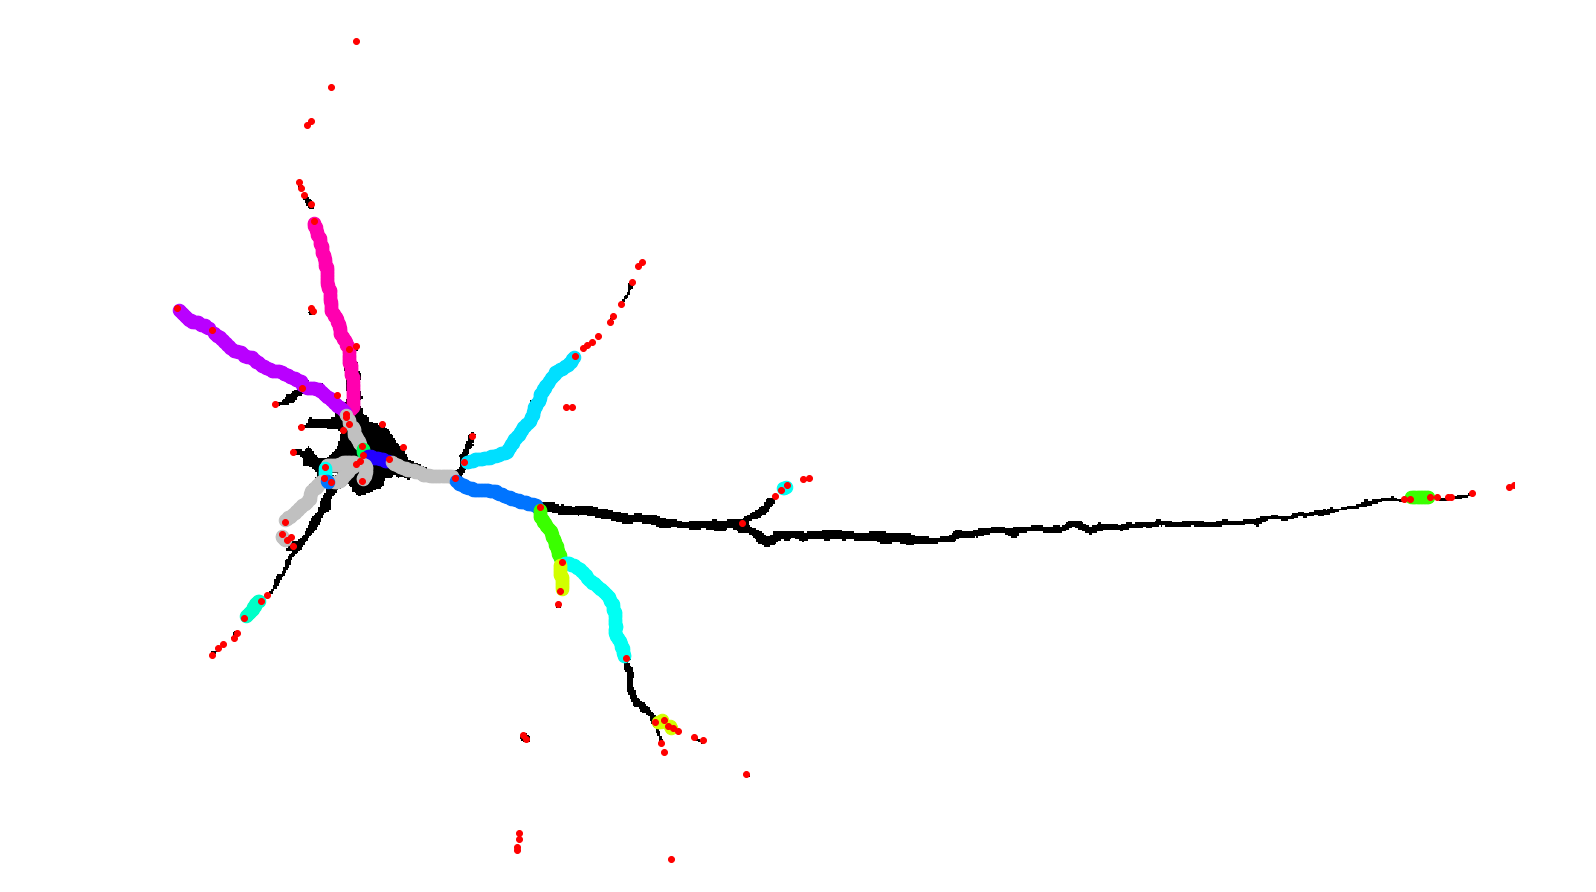
\includegraphics[height=1.35in]{Pictures/Porta18-3a1-phil-s10-v056-overmatches-3-antLabeled.png}
                \caption{Muestra N3 con sub/sobre asignaci\'on}
            \end{figure}
        \end{column}
    \end{columns}
    
    \begin{table}[h]
    \resizebox{0.65\textwidth}{!}{
        \begin{tabular}{|c|c|c|c|c|c|c|c|}
        \hline
              Muestra & C/Prop. & C/Prop.* & C/GT & C/GT* & F. Sub/Sobre asig. \\ \hline
            N1 & 1.6/59 & 3/66 & 1.6/24 & 3/24 & 1.4\\
            N2 & 4.6/34.8 & 6/34 & 4.6/29 & 6/29 & {\bf 8} \\
            N3 & 2/17.4 & 2/17 & 2/14 & 2/14 & {\bf 7.8}\\
            \hline
        \end{tabular}
        }
        \caption{(*) indica el mejor resultado de las 10 iteraciones}
    \end{table}
\end{frame}

\note[itemize]{
  \item En particular, al estudiar los filamentos propuestos por el algoritmo para el caso de neuronas, se observa que a\'un cuando los calces exactos son bajos, existen varios filamentos propuestos que se encuentran en un rango de 1 a 3 aristas faltantes o sobrantes, con respecto a un filamento correcto.
  
  \item as\'i, al incluir los filamentos propuestos con una diferencia de hasta 3 aristas, lo cual se refleja en las \'ultima columna de filamentos con sub o sobre asignaci\'on, se pueden encontrar varios filamentos candidatos descartados que se encuentran cercanos a lo definido por un experto, lo que indica para las neuronas puede ser necesario incluir un an\'alisis adicional durante la construcci\'on de soluciones mediante las hormigas.
  
  \item Lo anterior mejorar\'ia la cantidad de filamentos correctos, manteniendo el comportamiento del n\'umero de filamentos propuestos 
}

\begin{frame}{Resultados Generales (OE 4)}
\resizebox{0.85\textwidth}{!}{
    \begin{tabular}{|c|c|c|c|c|}
        \hline
        Figura & Config. & Fil. Correctos & Fil. Propuestos & $p$-value  \\ \hline
         4.1 & S1  & 6 & 5.9 & {\bf 1} \\
         4.2 & S2 & 5 & 8.5 & 0.003\\
         4.3 & MtP & 12 & 12.4 & {\bf 0.125}\\
         4.4 & MtP & 12 & 15 & 0\\
         4.5 & MtP & 5 & 5 & {\bf 1}\\
         4.6 & N & 24 & 60.2 & 0\\
         4.7 & N & 29 & 34.3 & 0\\
         4.8 & N & 14 & 17.6 & 0.003\\ 
         5.3b & MtP & 19 & 21 & 0.001\\
         5.3c & MtP & 23 & 29.4 & 0 \\
         5.9a & MtP & 13 & 14 & 0.001\\
         5.10a & MtP & 12 & 13.1 & 0\\
         \hline
    \end{tabular}
}
\end{frame}

\note[itemize]{
    
    \item En general, el hecho que el algoritmo propuesto no tenga diferencias estad\'isticamente significativas en 3 de las pruebas, as\'i como que presente un n\'umero de filamentos propuestos cercano a lo indicado por un experto en la mayor\'ia de los casos representa la capacidad del algoritmo de acotar el espacio de b\'usqueda de forma eficiente
    
    \item Es relevante destacar que la configuraci\'on predefinida para neuronas o para microt\'ubulos de planta no ha sido ajustada o sintonizada. Es probable que con una sintonización de par\'ametros, los resultados mejoren.
    
    \item SKIP Se defini\'o que La hip\'otesis nula (H0) fuese la no existencia de diferencia estad\'isticamente significativa entre el n\'umero de filamentos individualizados por el algoritmo propuesto y lo definido por el experto que realiz\'o la individualizaci\'on manual respectiva. En el caso de que el valor $p$ o {\it p-value} sea menor al 5\%, se rechaza H0. 
}